\documentclass[twocolumn]{article}
\usepackage{verbatim}
\usepackage{amsfonts}
\usepackage{geometry}
\usepackage{amsmath}
\usepackage{amsthm}
\usepackage{amssymb}
\usepackage{listings}
\usepackage{graphicx}
\usepackage{clrscode3e}
\usepackage{txfonts}
\usepackage{enumerate}
\usepackage{ctex}
\usepackage{txfonts}
\usepackage{fontspec-xetex}
\usepackage{float}
\geometry{top=2.5cm,bottom=2.5cm,left=2.5cm,right=2.5cm}
\setlength\parindent{0em}
\setmainfont{Times New Roman}
\newcommand*{\dif}{\mathop{}\!\mathrm{d}}
\begin{document}
	\title{问题求解(二)作业(第十五周)}\author{161180162 许致明}\maketitle
	\section*{TC第18章}
	\subsection*{18-1.1}
	若$t=1$,则内部节点至少有$t-1$个键。而此时$t-1=0$,说明某些内部节点没有代表任何键,这是对存储空间的浪费。
	\subsection*{18-1.4}
	若每个节点都包含$2t$个子节点,整个树内的节点数量最多。共有$$\sum_{i=0}^{h}(2t)^i=\frac{(2t)^{h+1}-1}{2t-1}$$
	每个节点至多有$2t-1$个键,则最多的键的个数为$(2t)^{h+1}-1$。
	\subsection*{18.2-3}
	一直向节点首个孩子前进,直至到达叶节点,此时就是最小元素。\par
	寻找一个节点的前继时,先找到这个节点。若它是叶节点,则直接返回它的父辈;若它不是,则返回它前面最大的孩子节点。
	\subsection*{18-2.4}
	节点个数为$2^{h+1}-1$,其中$h$为树的高度。又可知$n=2h+2^{h+1}+1$,则节点数量渐进为$\Theta(n)$。
	\subsection*{18-3.1}
	如图1所示:
	\begin{figure}[H]
		\centering
		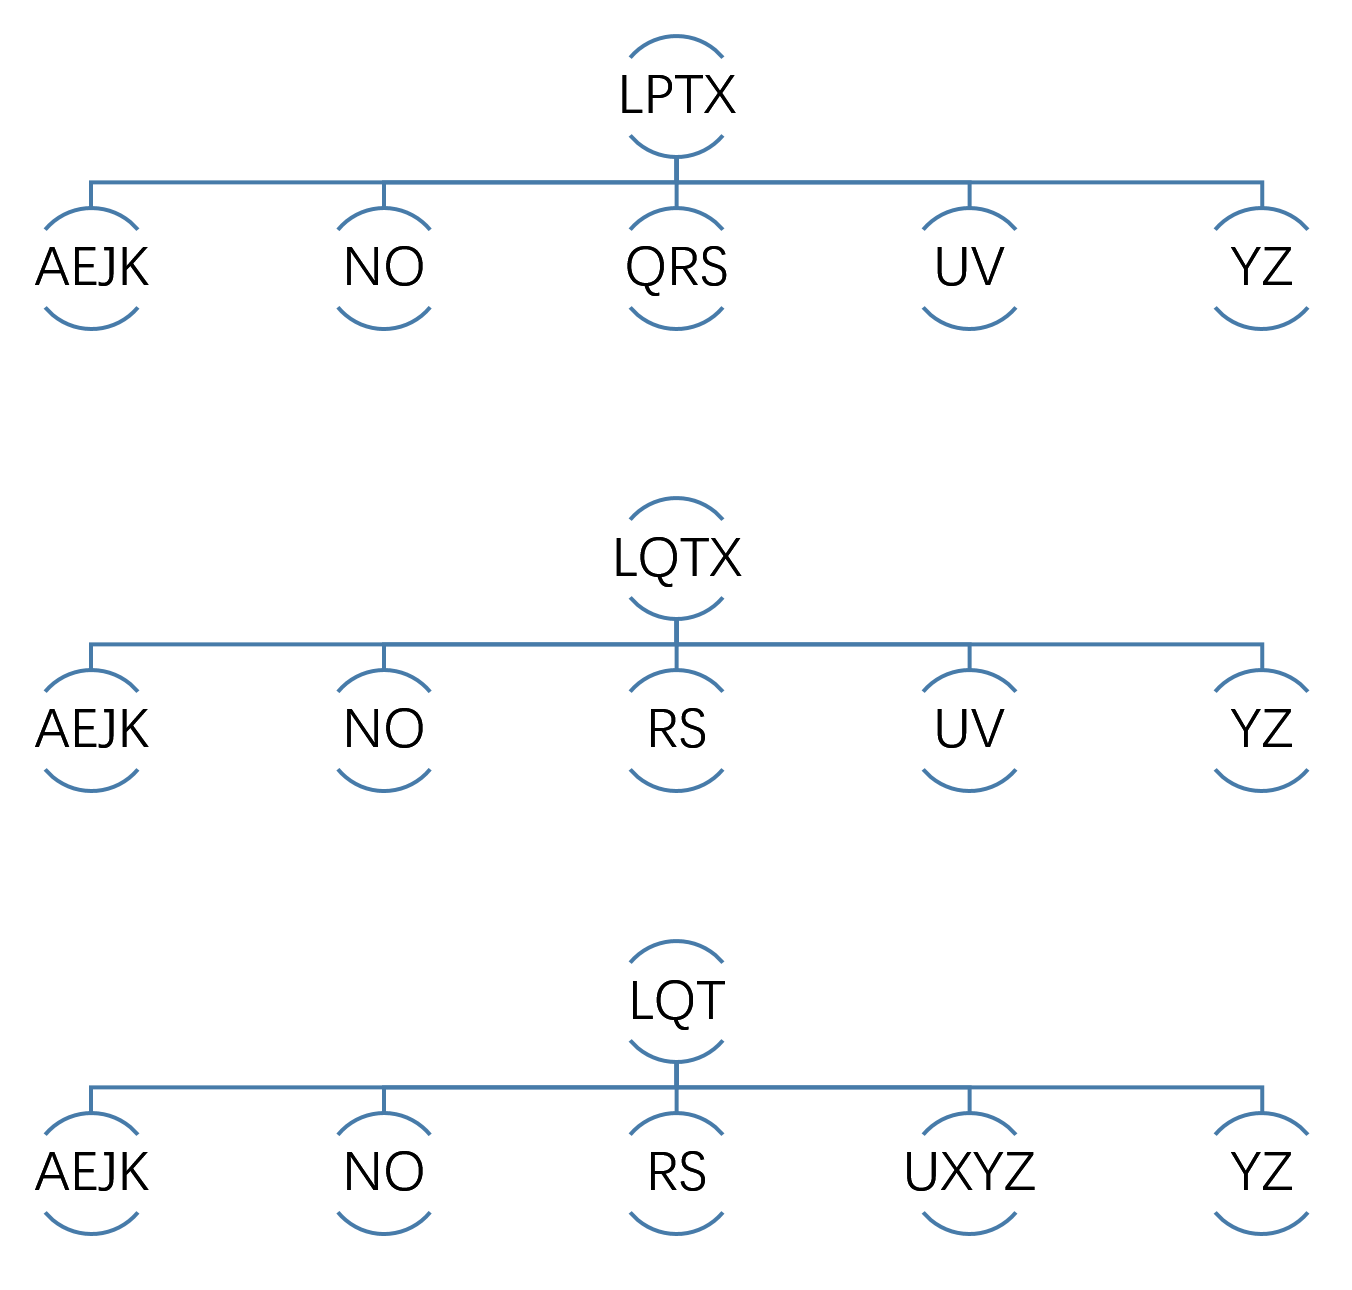
\includegraphics[width=1\linewidth]{14_1}
		\caption{18-3.1的删除结果}
	\end{figure}
\end{document}